%% Font size %%
\documentclass[11pt]{article}

%% Load the custom package
\usepackage{Mathdoc}

%% Numéro de séquence %% Titre de la séquence %%
\renewcommand{\centerhead}{Chap. 2 : Points, droites, segments}

\setlength{\parindent}{0pt}

\begin{document}

\textbf{Exercice 1 : Placer des points} \\
Place trois points A, B et C dans le cadre ci-dessous, en respectant
la notation vue en cours.

\begin{center}
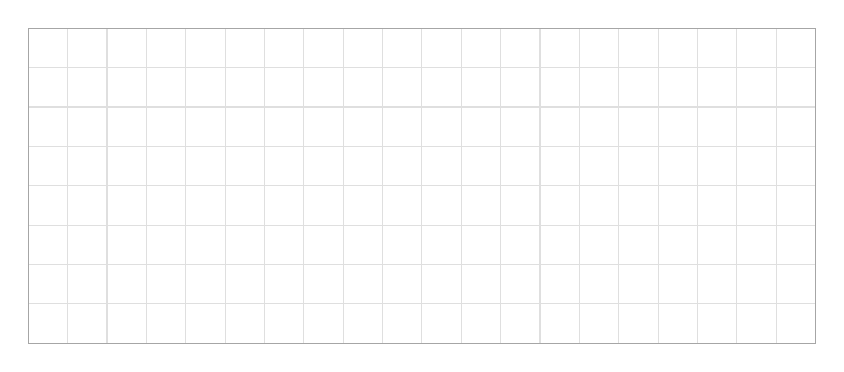
\begin{tikzpicture}
  \draw[gray!25,step=0.5] (0,0) grid (10,4);
  \draw[gray!70] (0,0) rectangle (10,4);
\end{tikzpicture}
\end{center}

\vspace{0.5cm}
\textbf{Exercice 2 : Lire une figure} \\
Observe la figure, puis entoure Vrai ou Faux.

\begin{center}
\begin{tikzpicture}[scale=1.1]
  \tkzDefPoint(0,0){D}
  \tkzDefPoint(3.4,2){E}
  \tkzDefPoint(6.8,0.5){F}
  \tkzDefPoint(1.7,-1.6){G}
  \tkzDrawPoints[shape=cross out,size=9](D,E,F,G)
  \tkzLabelPoints(D,E,F,G)
\end{tikzpicture}
\end{center}

\begin{enu}
\item Le point $E$ est représenté par une croix. \hfill Vrai\ /\ Faux
\item Il y a 4 points sur cette figure. \hfill Vrai\ /\ Faux
\item Le point $F$ est plus haut que le point $D$. \hfill Vrai\ /\ Faux
\end{enu}

\vspace{0.5cm}
\textbf{Exercice 3 : Trouve les erreurs} \\
Certains points ci-dessous ne sont pas notés correctement. Entoure-les tous.

\begin{center}
\begin{tikzpicture}[scale=1]
  \tkzDefPoint(0,0){A}
  \tkzDefPoint(4.8,0){B}
  \tkzDefPoint(9.6,0){E}
  \tkzDrawPoints[shape=cross out,size=9](A,B,E)
  \tkzLabelPoints(A,B,E)
  \fill (2.4,0) circle (3.5pt);
  \node[above] at (2.4,0.2) {$c$};
  \fill (7.2,0) circle (3.5pt);
  \node[above] at (7.2,0.2) {$D$};
  \draw[thick] (12,0) circle (3.5pt);
  \node[above] at (12,0.2) {$f$};
\end{tikzpicture}
\end{center}

\end{document}

%%% Local Variables:
%%% mode: LaTeX
%%% TeX-master: t
%%% End:
